\documentclass[tikz,border=8pt]{standalone}
\usepackage{amsmath,amssymb}
\usetikzlibrary{arrows.meta,calc,decorations.pathreplacing,patterns,shapes.geometric,positioning,shadings}

\begin{document}
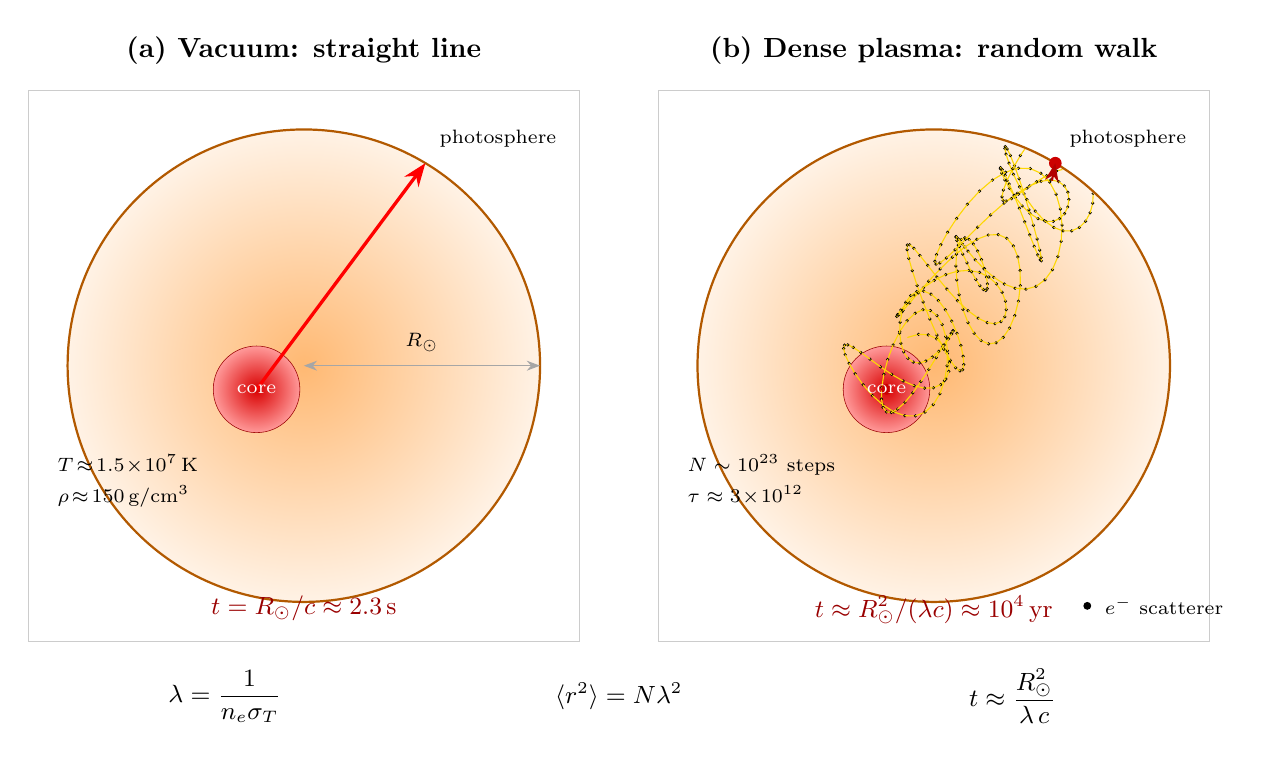
\begin{tikzpicture}[>=Stealth,font=\small]

% =====================================================
% Two side-by-side panels comparing photon trajectories
% Left panel: vacuum straight-line path
% Right panel: random walk through plasma
% =====================================================

% ---- Panel titles ----
\node[font=\bfseries] at (3.5,7.5) {(a) Vacuum: straight line};
\node[font=\bfseries] at (11.5,7.5) {(b) Dense plasma: random walk};

% =====================================================
% PANEL 1 : Vacuum straight-line trajectory
% =====================================================
\begin{scope}[shift={(0,0)}]
  \draw[gray!40] (0,0) rectangle (7,7);

  % Sun disk with pale orange radial shading
  \shade[inner color=orange!55,outer color=orange!10]
    (3.5,3.5) circle (3.0);
  \draw[orange!70!black,thick] (3.5,3.5) circle (3.0);

  % Core
  \shade[inner color=red!85!black,outer color=red!40]
    (2.9,3.2) circle (0.55);
  \draw[red!60!black,very thin] (2.9,3.2) circle (0.55);

  % Red straight line from core to surface
  \draw[red,very thick,->] (2.9,3.2) -- (5.044,6.072);

  \node[font=\scriptsize,white] at (2.9,3.2) {core};

  \node[font=\scriptsize,anchor=north west] at (0.25,2.5)
    {$T\!\approx\!1.5\!\times\!10^{7}$\,K};
  \node[font=\scriptsize,anchor=north west] at (0.25,2.1)
    {$\rho\!\approx\!150$\,g/cm$^3$};

  \node[font=\scriptsize,anchor=south west] at (5.1,6.15)
    {photosphere};

  \draw[<->,gray!70] (3.5,3.5) -- ++(0:3.0);
  \node[font=\scriptsize,anchor=south] at (5.0,3.55) {$R_\odot$};

  \node[font=\small,red!60!black,anchor=north] at (3.5,0.7)
    {$t = R_\odot/c \approx 2.3\,\text{s}$};

\end{scope}

% =====================================================
% PANEL 2 : Random walk trajectory
% Build path incrementally by drawing one segment at a time inside \foreach.
% Uses global let to carry (curx,cury) between iterations.
% =====================================================
\begin{scope}[shift={(8,0)}]
  \draw[gray!40] (0,0) rectangle (7,7);

  % Sun disk
  \shade[inner color=orange!55,outer color=orange!10]
    (3.5,3.5) circle (3.0);
  \draw[orange!70!black,thick] (3.5,3.5) circle (3.0);

  % Core
  \shade[inner color=red!85!black,outer color=red!40]
    (2.9,3.2) circle (0.55);
  \draw[red!60!black,very thin] (2.9,3.2) circle (0.55);

  % ---- Random walk path ----
  % Build a polyline parameterized by index i in [0,300].
  % Core at (2.9,3.2), surface target (5.044,6.072).
  % Use small angular multipliers to avoid pgfmath dimension overflow
  % (TeX dimension max ~16383 pt; keep \i * mult < ~5000).
  \begin{scope}
    \clip (3.5,3.5) circle (2.98);
    \foreach \i in {0,...,299}{
      \pgfmathsetmacro{\aoneA}{\i*13.1}
      \pgfmathsetmacro{\atwoA}{\i*9.3}
      \pgfmathsetmacro{\athreeA}{\i*7.9}
      \pgfmathsetmacro{\afourA}{\i*17.7}
      \pgfmathsetmacro{\afiveA}{\i*11.1}
      \pgfmathsetmacro{\asixA}{\i*3.3}
      \pgfmathsetmacro{\xa}{2.9+0.00715*\i+0.48*sin(\aoneA)+0.27*cos(\atwoA)+0.18*sin(\athreeA)}
      \pgfmathsetmacro{\ya}{3.2+0.00957*\i+0.48*cos(\afourA)+0.27*sin(\afiveA)+0.18*cos(\asixA)}
      \pgfmathtruncatemacro{\j}{\i+1}
      \pgfmathsetmacro{\aoneB}{\j*13.1}
      \pgfmathsetmacro{\atwoB}{\j*9.3}
      \pgfmathsetmacro{\athreeB}{\j*7.9}
      \pgfmathsetmacro{\afourB}{\j*17.7}
      \pgfmathsetmacro{\afiveB}{\j*11.1}
      \pgfmathsetmacro{\asixB}{\j*3.3}
      \pgfmathsetmacro{\xb}{2.9+0.00715*\j+0.48*sin(\aoneB)+0.27*cos(\atwoB)+0.18*sin(\athreeB)}
      \pgfmathsetmacro{\yb}{3.2+0.00957*\j+0.48*cos(\afourB)+0.27*sin(\afiveB)+0.18*cos(\asixB)}
      \draw[yellow!75!orange,line width=0.4pt,line cap=round] (\xa,\ya) -- (\xb,\yb);
      \fill[black] (\xb,\yb) circle (0.022);
    }
  \end{scope}

  % Highlight core start and surface end
  \fill[red!80!black] (2.9,3.2) circle (0.07);
  \fill[red!80!black] (5.044,6.072) circle (0.08);
  \draw[->,red!70!black,thick] (5.0,5.85) -- (5.044,6.072);

  \node[font=\scriptsize,white] at (2.9,3.2) {core};
  \node[font=\scriptsize,anchor=south west] at (5.1,6.15)
    {photosphere};

  \node[font=\scriptsize,anchor=north west] at (0.25,2.5)
    {$N \sim 10^{23}$ steps};
  \node[font=\scriptsize,anchor=north west] at (0.25,2.1)
    {$\tau \approx 3\!\times\!10^{12}$};

  \node[font=\small,red!60!black,anchor=north] at (3.5,0.7)
    {$t \approx R_\odot^{2}/(\lambda c) \approx 10^{4}\,\text{yr}$};

  \fill[black] (5.45,0.45) circle (0.05);
  \node[font=\scriptsize,anchor=west] at (5.55,0.45) {$e^{-}$ scatterer};

\end{scope}

% =====================================================
% Formula row (bottom)
% =====================================================
\node[font=\small] at (2.5,-0.7)
  {$\lambda = \dfrac{1}{n_{e}\sigma_{T}}$};
\node[font=\small] at (7.5,-0.7)
  {$\langle r^{2}\rangle = N\lambda^{2}$};
\node[font=\small] at (12.5,-0.7)
  {$t \approx \dfrac{R_\odot^{2}}{\lambda\, c}$};

\end{tikzpicture}
\end{document}
